\section{Evaluation}
\label{sec:evaluation}
The new language has been evaluated through a prototype implementation that builds on 
the ASTRA \cite{DBLP:conf/prima/CollierRL15} language. This prototype, which is compatible
with pure ASTRA code, is used to reimplement part of an existing solution for the Minority 
Game \cite{moro2004minority}. Interpreter cycle timings are then captured to develop an initial
understanding of how the new language performs.

As can be seen in the  snippet of code below,the implementation of the {\aser} prototype is 
syntactically different to the example provided in section \ref{sec:proposal}. This reflects 
the syntactic approach adopted in ASTRA. It does not impact the associated semantics.

{\small
\begin{verbatim}
g-rule +!g() : c <: gc { 
  body {
    // main plan body goes here...
    a; b; !g1(); !!g2();
  }

  /* e-plans */
  rule +e1 : c1 { b1; }
  rule +e2 : c2 { b2; }
}
\end{verbatim}}

\begin{figure}[!bh]
\centering
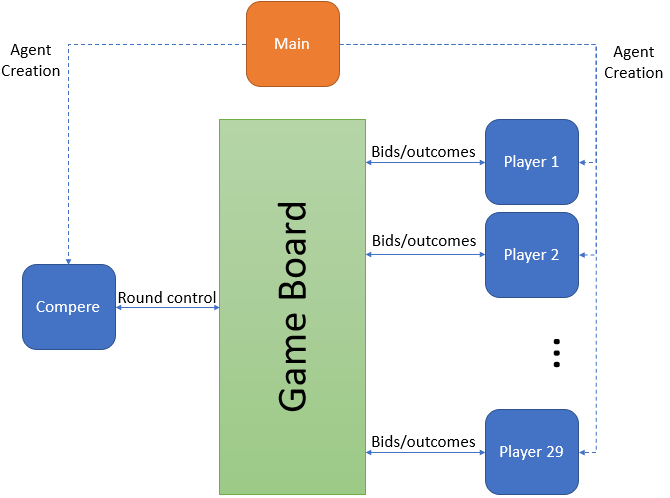
\includegraphics[height=2in, width=2.5in]{mg.png}
\caption{Minority Game Agent Architecture}
\label{fig:mgagents}
\end{figure}

\subsection{Minority Game}
\label{minority}
The Minority Game is a well known model for evaluating collective behaviour of agents competing 
for finite resources \cite{moro2004minority}. In a nutshell, the game involves an odd number of
agents competing for a resource over a series of rounds. For a round, each agent makes a binary
decision (yes/no). At the end of the round, the bids are counted, and the agents that are in the
minority win. The game has been applied mainly in the area of modelling financial markets \cite{??}.

To provide an initial evaluation of {\aser}, we adapt an existing ASTRA-based implementation of 
the Minority Game MG). As is shown in figure \ref{fig:mgagents}, the implementation consists of
3 types of agent: the \emph{compere} agent, who is responsible for managing the game (starting 
rounds, evaluating bids, ...); the \emph{player} agent, who implements a set of MG strategies; 
and the \emph{main} agent, which is responsible for configuring the game (creating and configuring
the compere and player agents).

The existing implementation currently consists of 10 plans. Two of the plans are generic and are
used for configuration. Another plan implements the bidding behaviour, delegating to a 
\verb|!select_bid(...)| sub goal that can be contextually selected based on the current strategy.
Of the remaining plans: four relate to the best play strategy; one relates to a random strategy;
and two relate to a sticky strategy.

In the {\aser} implementation, we reduce this to 4 of the new g-rules: one to handle configuration
and one for each of the strategies. The code below illustrates this new model through the
revised implementation of the best play strategy.

{\small
\begin{verbatim}
  g-rule +!win("bestplay", [int t, int h]) <: false {
    body {
      !setup_tactic(t);
    }

    rule +!setup_tactic(0) {}
    rule +!setup_tactic(int t2) {
      list hist = [];
			
      // construct a random history
      int i=0;
      while (i<h) {
        hist = hist + [M.randomInt() % 2];
        i++;
      }
			
      +strategy(t2, hist, M.randomInt() % 2);
      +score(t2, 0);
		
      !setup_tactic(t2-1);
    }
		
    rule $A.event("play", []) { 
      list history = A.results();
			
      int max_len = -1;
	  int max_choice = -1;
	  int max_score = -1;
	  foreach (strategy(int s, list hist, int c) & score(s, int sc)) {
	    int len = A.match(history, hist);
        if ((len > max_len) | ((len == max_len) & (max_score < sc))) {
          max_choice = c;
          max_score = sc;
          max_len = len;
        }
      }
		
      A.bid(max_choice);
    }
		
    rule $A.event("winner", [int bid]) {
	  foreach (strategy(int s, list hist, bid) & score(s, int sc)) {
        -+score(s, sc+1);
      }
    }
  }
\end{verbatim}}

Explain this code a bid...

\subsection{Preliminary Analysis}
\label{performance}


So, I have used the minority game example to try to get some timings for the impact of performance. I did this by reimplementing the player in ASER and leaving the rest the same.

I have done around 5 runs with each language. For each run, I have used the ASTRA main/compere agents and have used 29 player agents competing over 1000 rounds. All use the best-play strategy with the same history/strategy settings (see the cited paper if you want to understand the strategy better). I have then done some basic analysis on the results:

ASTRA averages around 0.004ms per cycle (but uses only around 50,000 cycles due to a dynamic scheduler that suspends the agent when the event+intention queues are empty).

ASER averages around 0.002ms per cycle (but uses around 500,000 cycles because the dynamic scheduler does not work for ASER).

This means that per cycle, ASER is approx 5 times slower than ASTRA in this example

That said, I also captured the overall duration of the game. There was no impact on this - both take around 19 seconds to complete

I can do this up as an experiment, with 5 runs per system, and calculate the average time per run / overall + the average number of cycles per run / overall